\documentclass[a4paper,10pt]{report}
\usepackage[utf8]{inputenc}
\usepackage{textcomp}
\usepackage{graphicx}
\usepackage{parskip}
\usepackage{hyperref}
\usepackage{color}
\usepackage{pdfpages}
\usepackage{pgf}
\usepackage{tikz}
\usepackage{amsfonts}
\usepackage{float}
\restylefloat{table}
\usetikzlibrary{arrows,automata}

\begin{document}
\begin{titlepage}
			\begin{center}
			\textsc{\LARGE {INSYGHT Lab}}\\[1cm]
			\rule{\linewidth}{0.5mm} \\[0.4cm]

			{\Huge \bfseries RoboTutor Project}\\[0.15cm]

			\rule{\linewidth}{0.5mm} \\
			\textsc{\large{Interactive robot teacher}}
			
			\vskip 2 cm
			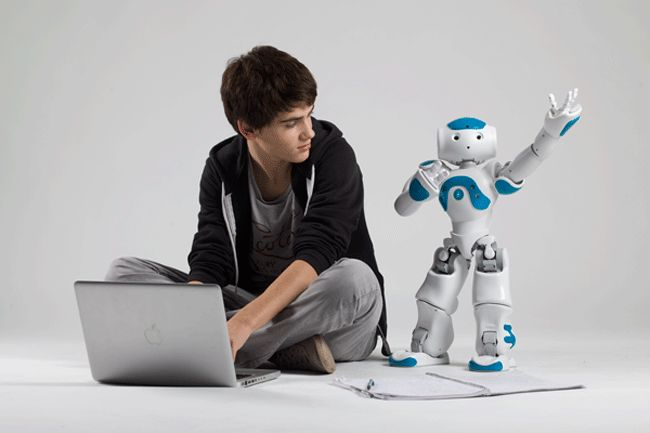
\includegraphics[scale=1.5]{nao02.jpg}
			\vskip 1 cm
			\rule{\linewidth}{0.5mm}
			
			\vskip 0.5 cm
			
			\begin{minipage}{0.4\textwidth}
				\begin{flushleft} \large
					\emph{Authors:}\\
					\begin{tabular}{l}
						M. De Vries (4011562) \\
						A. Drif (4030532) \\
						H. Gaiser (4007891) \\
						J.E.T. Tan (4032918)\\
						P. Veldhuisen (4153448)\\
					\end{tabular}
				\end{flushleft}
			\end{minipage}
			\hspace{1cm}
			\begin{minipage}{0.4\textwidth}
				\begin{flushright} \large
					\emph{Supervisor:} \\
					Dr. K. Hindriks
				\end{flushright}
			\end{minipage}
			
			\vskip 0.5 cm
			
			\rule{\linewidth}{0.5mm}
			\end{center}
\end{titlepage}
\setcounter{secnumdepth}{0}
\tableofcontents

\section{Introduction}
\label{sec:intro}

In this project we will attempt to create a robotic teaching assistent, who will assist a lecturer for five minutes during lectures with robotics related topics.

\section{Features}
\label{sec:features}
See below here for a road map of the project.
\begin{description}
 \item Must haves:
	\begin{itemize}
		\item Lecture scripts
			\begin{description}
				\item Text
				\item Behaviours
				\item Slides
			\end{description}
		\item 'Random' pose changes
		\item Audio streaming to speakers
		\item Teacher interaction
		\item Point at slides
		\item Do not fall of platform
		\item Hold quizzes
			\begin{description}
				\item Clicker support
				\item Respond to answers
			\end{description}
	\end{itemize}

 \item Should haves:
	\begin{itemize}
		\item Lecture script GUI
		\item Recognizing raised hands
		\item Noise level detection
		\item Mood indicator
	\end{itemize}

 \item Could haves:
	\begin{itemize}
		\item Remote image processing
		\item Laptop recognition
		\item Food recognition
		\item Cluster quiz answers
		\item Subtitles
	\end{itemize}

 \item Would haves:
	\begin{itemize}
		\item World peace
	\end{itemize}
\end{description}

\section{Tickets}
\begin{description}
	\item Script engine: \textit{Anass en Maarten}
		\begin{itemize}
			\item Design script grammar \textit{2}
			\item Implement parser \textit{3}
			\item Design script engine API \textit{1}
			\item Implement script engine \textit{4}
		\end{itemize}
	\item Pose changes: \textit{Pim en Hans}
		\begin{itemize}
			\item Design poses in choreographe \textit{2}
			\item Implement 'random' pose changer \textit{2}
		\end{itemize}
	\item Remote audio playback: \textit{Maarten en Jethro}
		\begin{itemize}
			\item Access robot (telnet/ssh) \textit{2} \textbf{DONE}
			\item Research audio streaming / alternative \textit{5}
		\end{itemize}
	\item Teacher interaction: \textit{Anass en Hans}
		\begin{itemize}
			\item Recognize voices \textit{4}
			\item Teacher interruption \textit{2}
		\end{itemize}
	\item Slides: \textit{Jethro en Pim}
		\begin{itemize}
			\item Research slides control \textit{2}
			\item Point at slides \textit{2}
		\end{itemize}
	\item Quizzes: \textit{Anass, Jethro en Maarten}
		\begin{itemize}
			\item Research clicker system \textit{4}
			\item Implement clicker support \textit{4}
			\item Design feedback mechanism \textit{3}
			\item Implement feedback system \textit{1}
			\item Clicker localisation \textit{1}
		\end{itemize}
	\item Remote control GUI: \textit{Hans en Jethro}
		\begin{itemize}
			\item Design RC GUI \textit{3}
			\item Implement RC GUI \textit{5}
		\end{itemize}
	\item Class interaction: \textit{Anass, Hans en Pim}
		\begin{itemize}
			\item Noise detection \textit{2} \textit{Pim}
			\item Noise handling \textit{2} \textit{Pim}
			\item Raised hand recognition \textit{4} \textit{Hans}
			\item Design mood poses \textit{2} \textit{Anass}
			\item Mood indicator \textit{2} \textit{Anass}
		\end{itemize}
\end{description}
			
\end{document}
